\chapter{Całki powierzchniowe i miara Hausdorffa}
\label{ma2:ch:surface-integrals}

Całka po krzywej z rozdziału \ref{ma2:ch:line-integrals}
wykorzystuje długość, a całka po zbiorze w $\R^n$
z rozdziału \ref{ma2:ch:multiple-integrals} wykorzystuje
$n$-wymiarową objętość. Teraz rozważymy całkowanie
względem $k$-wymiarowej objętości podrozmaitości
w $\R^n$, gdzie $1\le k\le n$.
Nie potrzebujemy ogólnej teorii rozmaitości
riemannowskich. Metrykę przestrzeni otaczającej
stanowi zwykła metryka euklidesowa.

\section{Intuicja: pole fragmentu a pole jego rzutu}

Mały prostokąt w dziedzinie parametryzacji
$\sigma:U\subseteq\R^k\to\R^n$ przechodzi w mały
fragment podrozmaitości. W pierwszym przybliżeniu
jest to równoległościan rozpięty przez kolumny
$D\sigma(u)$ pomnożone przez długości boków
prostokąta. Z rozdziału \ref{ma2:ch:manifold-calculus}
znamy $k$-wymiarowy jakobian
\[
 J_k\sigma(u)=\sqrt{\det(D\sigma(u)^{\mathsf T}D\sigma(u))}.
\]
Jest on czynnikiem zmiany lokalnej objętości,
a nie wyznacznikiem prostokątnej macierzy pochodnej.
Dla $k=1$ otrzymujemy normę prędkości, a dla $k=n$
moduł zwykłego wyznacznika. Gdy $k<n$, miara
$\lambda_n$ nie mierzy pola podrozmaitości:
jej miara $n$-wymiarowa jest zerowa, jak wynika
z lematu \ref{ma2:lem:surface-lower-dimension}
i przeliczalnego pokrycia lokalnymi parametryzacjami.
Potrzebujemy miary odpowiedniego wymiaru.

\begin{figure}[htbp]
\centering
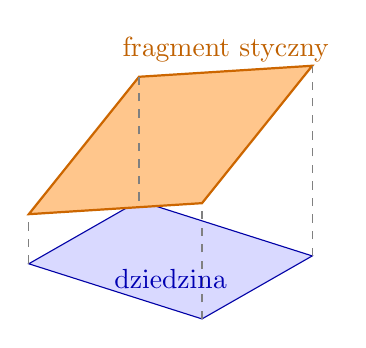
\begin{tikzpicture}[x={(1.1cm,-.35cm)},y={(-.7cm,-.4cm)},z={(0cm,1.05cm)}]
\fill[blue!15] (0,0,0)--(2,0,0)--(2,2,0)--(0,2,0)--cycle;
\draw[blue!65!black] (0,0,0)--(2,0,0)--(2,2,0)--(0,2,0)--cycle;
\fill[orange!45] (0,0,1.5)--(2,0,2.3)--(2,2,1.4)--(0,2,.6)--cycle;
\draw[orange!80!black,thick] (0,0,1.5)--(2,0,2.3)--(2,2,1.4)--(0,2,.6)--cycle;
\foreach \x/\y/\z in {0/0/1.5,2/0/2.3,2/2/1.4,0/2/.6}
 \draw[gray,dashed] (\x,\y,0)--(\x,\y,\z);
\node[blue!70!black,below] at (1,1,0) {dziedzina};
\node[orange!75!black,above] at (1,0,1.9) {fragment styczny};
\end{tikzpicture}
\caption{Pole fragmentu stycznego może być większe
od pola rzutu na płaszczyznę parametrów.}
\label{ma2:fig:surface-projection}
\end{figure}

\section{Miara Hausdorffa i liniowa zmiana pola}

Stosujemy miarę $\mathcal H^k$ unormowaną tak, by
na $\R^k$ pokrywała się na zbiorach borelowskich
z $\lambda_k$. Konstrukcję, borelowską mierzalność,
normalizację oraz nierówność Lipschitzowską
udowodniono w
\atlasref{ME-26::thm:hausdorff-borel-26}{ME 26},
\atlasref{ME-26::thm:hausdorff-calibration-26}{twierdzeniu o kalibracji}
i \atlasref{ME-26::thm:hausdorff-lipschitz-26}{twierdzeniu o skalowaniu}.
W szczególności izometrie zachowują $\mathcal H^k$,
a dla odwzorowania $L$-Lipschitzowskiego $F$
mamy $\mathcal H^k(F(A))\le L^k\mathcal H^k(A)$.
Miara obliczona w podprzestrzeni metrycznej jest
taka sama jak w przestrzeni otaczającej: pokrycia
w przestrzeni otaczającej można przeciąć z podprzestrzenią,
nie zwiększając średnic; pokrycia w podprzestrzeni
są zarazem pokryciami w przestrzeni otaczającej.

\begin{lemat}[Liniowy wzór na pole]
\label{ma2:lem:surface-linear-area}
Niech $A:\R^k\to\R^n$ będzie różnowartościowym
odwzorowaniem liniowym. Dla borelowskiego
$B\subseteq\R^k$ zachodzi
\[
 \mathcal H^k(A(B))=\sqrt{\det(A^{\mathsf T}A)}\lambda_k(B).
\]
\end{lemat}
\begin{proof}
Wybierzmy izometrię liniową $Q:\R^k\to A(\R^k)$
za pomocą bazy ortonormalnej obrazu.
Wówczas $A=QR$ z odwracalną macierzą $R=Q^{\mathsf T}A$.
Z niezmienniczości izometrycznej i kalibracji
$\mathcal H^k(A(B))=\lambda_k(R(B))$.
Z afinicznego wzoru \ref{ma2:ex:multiple-affine}
jest to $|\det R|\lambda_k(B)$.
Ponieważ $A^{\mathsf T}A=R^{\mathsf T}R$, otrzymujemy tezę.
\end{proof}

\section{Wzór na pole dla parametryzacji klasy \texorpdfstring{$C^1$}{C\textasciicircum 1}}

\begin{twierdzenie}[Wzór na pole dla zanurzenia]
\label{ma2:thm:surface-area}
Niech $1\le k\le n$, $U\subseteq\R^k$ będzie
otwarty, a $\sigma:U\to\R^n$ zanurzeniem klasy $C^1$,
to znaczy różnowartościową immersją będącą
homeomorfizmem na obraz. Dla borelowskiego $B\subseteq U$
\[
 \mathcal H^k(\sigma(B))=\int_B J_k\sigma(u)\,
 \mathrm d\lambda_k(u).
\]
\end{twierdzenie}
\begin{proof}
Obraz $U$ jest przeliczalną sumą zbiorów zwartych:
$U$ ma wyczerpanie zbiorami zwartymi, a $\sigma$
jest ciągła. Jest więc borelowski w $\R^n$.
Homeomorfizm na obraz zapewnia borelowską
mierzalność $\sigma(B)$.

Ustalmy $0<\varepsilon<1$ i $u_0\in U$.
Niech $A=D\sigma(u_0)$. Ponieważ $A$ jest
różnowartościowe, istnieje $m>0$ takie, że
$\|Ah\|_2\ge m\|h\|_2$ dla każdego $h$;
można wziąć minimum $\|Ah\|_2$ na sferze jednostkowej.
Z ciągłości pochodnej i dodatniości jakobianu
wybieramy otwartą kulę $V$ o środku $u_0$,
z domknięciem w $U$, na której
\[
 \|D\sigma(u)-A\|\le\varepsilon m,\qquad
 (1-\varepsilon)J_k\sigma(u_0)\le J_k\sigma(u)
 \le(1+\varepsilon)J_k\sigma(u_0).
\]
Dla $u,v\in V$ odcinek łączący te punkty należy do $V$.
Nierówność wartości średniej zastosowana do
odwzorowania $w\mapsto\sigma(w)-Aw$ na odcinku
od $v$ do $u$ (jego pochodna wzdłuż odcinka ma
normę co najwyżej $\varepsilon m\|u-v\|_2$) daje
\[
 \|\sigma(u)-\sigma(v)-A(u-v)\|_2
 \le\varepsilon m\|u-v\|_2
 \le\varepsilon\|A(u-v)\|_2.
\]
Stąd
\[
 (1-\varepsilon)\|A(u-v)\|_2
 \le\|\sigma(u)-\sigma(v)\|_2
 \le(1+\varepsilon)\|A(u-v)\|_2.
\]
Odwzorowanie $Au\mapsto\sigma(u)$ i jego odwrotność
są Lipschitzowskie na odpowiednich obrazach.
Nierówność dla miary Hausdorffa i
lemat \ref{ma2:lem:surface-linear-area} dają
dla każdego borelowskiego $C\subseteq V$
\[
 (1-\varepsilon)^kJ_k\sigma(u_0)\lambda_k(C)
 \le\mathcal H^k(\sigma(C))
 \le(1+\varepsilon)^kJ_k\sigma(u_0)\lambda_k(C).
\]
Porównując z oszacowaniem jakobianu, otrzymujemy
\[
 \frac{(1-\varepsilon)^k}{1+\varepsilon}
 \int_C J_k\sigma(u)\,\mathrm d\lambda_k(u)
 \le\mathcal H^k(\sigma(C))
 \le\frac{(1+\varepsilon)^k}{1-\varepsilon}
 \int_C J_k\sigma(u)\,\mathrm d\lambda_k(u).
\]
Kule $V$ tworzą pokrycie otwarte $U$.
Z drugiego aksjomatu przeliczalności wybieramy
podpokrycie przeliczalne $(V_j)_{j\ge1}$.
Zbiory $C_j=B\cap(V_j\setminus\bigcup_{i<j}V_i)$
są borelowskie, parami rozłączne i pokrywają $B$.
Różnowartościowość $\sigma$ zapewnia rozłączność
ich obrazów. Sumujemy ostatnie nierówności dzięki
przeliczalnej addytywności obu miar. Jeżeli całka
jest nieskończona, dolne oszacowanie daje od razu
nieskończoną miarę obrazu. W przeciwnym razie
przechodzimy z $\varepsilon$ do zera.
\end{proof}

\begin{wniosek}[Ważony wzór na pole]
\label{ma2:cor:surface-weighted-area}
Przy założeniach twierdzenia \ref{ma2:thm:surface-area}
dla nieujemnej funkcji borelowskiej
$f:\sigma(B)\to[0,\infty]$ lub rzeczywistej funkcji
borelowskiej całkowalnej względem $\mathcal H^k$
\[
 \int_{\sigma(B)} f(x)\,\mathrm d\mathcal H^k(x)
 =\int_B f(\sigma(u))J_k\sigma(u)\,\mathrm d\lambda_k(u).
\]
\end{wniosek}
\begin{proof}
Dla funkcji charakterystycznych zbiorów borelowskich
jest to twierdzenie \ref{ma2:thm:surface-area} zastosowane
do ich przeciwobrazów. Liniowość daje wzór dla
nieujemnych funkcji prostych, a twierdzenie o zbieżności
monotonicznej dla dowolnych funkcji nieujemnych.
W przypadku funkcji ze znakiem stosujemy wynik
do części dodatniej i ujemnej; obie całki są skończone.
\end{proof}

\section{Całka na podrozmaitości i niezależność od map}

\begin{definicja}[Całka powierzchniowa pierwszego rodzaju]
\label{ma2:def:surface-integral}
Niech $M\subseteq\R^n$ będzie $k$-wymiarową
podrozmaitością klasy $C^1$ bez brzegu,
a $E\subseteq M$ zbiorem borelowskim.
Dla funkcji borelowskiej nieujemnej lub całkowalnej
względem $\mathcal H^k$ definiujemy całkę skalarną
po $E$ jako $\int_E f(x)\,\mathrm d\mathcal H^k(x)$.
Dla $k=2$ jest to klasyczna całka powierzchniowa
pierwszego rodzaju.
\end{definicja}
Każda podrozmaitość ma przeliczalne pokrycie
lokalnymi parametryzacjami $\sigma_j:U_j\to M$,
gdyż jako podprzestrzeń $\R^n$ spełnia drugi
aksjomat przeliczalności. Ich obrazy $M_j$
są borelowskie jak w dowodzie
\ref{ma2:thm:surface-area}, więc $M$ jest borelowski.
Dzieląc $E$ na rozłączne zbiory
$E_j=E\cap(M_j\setminus\bigcup_{i<j}M_i)$
otrzymujemy ze wzoru ważonego
\[
 \int_E f(x)\,\mathrm d\mathcal H^k(x)
 =\sum_j\int_{\sigma_j^{-1}(E_j)}
 f(\sigma_j(u))J_k\sigma_j(u)\,\mathrm d\lambda_k(u).
\]
Dla funkcji ze znakiem szereg jest bezwzględnie
zbieżny, bo suma modułów jego składników
nie przekracza całki z $|f|$.
Wynik nie zależy od pokrycia ani kolejności,
ponieważ jest równy jednej całce względem $\mathcal H^k$.
Lokalnie niezależność wynika również z reguły
\ref{ma2:prop:gram-change} i twierdzenia
\ref{ma2:thm:multiple-change} o zamianie zmiennych.
Orientacja nie wpływa na wartość całki skalarnej.

\begin{wniosek}[Lokalna skończoność miary powierzchniowej]
\label{ma2:cor:surface-local-finite}
Każdy punkt podrozmaitości klasy $C^1$ bez brzegu
ma względnie otwarte otoczenie o skończonej
mierze $\mathcal H^k$. W szczególności każdy
zwarty podzbiór podrozmaitości ma skończoną
miarę $\mathcal H^k$, a miara ograniczona do
podrozmaitości jest $\sigma$-skończona.
\end{wniosek}
\begin{proof}
Dla ustalonego $p\in M$ wybieramy parametryzację
lokalną $\sigma:U\to M$ z $p=\sigma(u_0)$,
a następnie kulę $V$ o środku $u_0$ i domknięciu
zwartym zawartym w $U$. Ciągły jakobian $J_k\sigma$
jest ograniczony na $\overline V$, więc
z \ref{ma2:thm:surface-area}
\[
 \mathcal H^k(\sigma(V))
 \le\lambda_k(V)\max_{\overline V}J_k\sigma<\infty.
\]
Takie otoczenia pokrywają $M$. Zwarty podzbiór
pokrywamy skończenie wieloma z nich, a całe $M$
przeliczalnie wieloma dzięki drugiemu aksjomatowi
przeliczalności.
\end{proof}

Wzór na pole obowiązuje również dla zbiorów
i funkcji mierzalnych względem uzupełnionych
miar. Istotnie, w przypadku zanurzenia
$J_k\sigma>0$ wszędzie, więc dla borelowskiego
$A\subseteq U$ zachodzi
$\mathcal H^k(\sigma(A))=0$ wtedy i tylko wtedy,
gdy $\lambda_k(A)=0$. W kierunku nietrywialnym
rozkładamy $A$ na przeliczalną sumę zbiorów
$A\cap\{J_k\sigma\ge1/m\}$, $m\ge1$.
Zatem zanurzenie i jego odwrotność przenoszą
podzbiory borelowskich zbiorów miary zero
na zbiory miary zero w odpowiednich miarach.
Każdy zbiór mierzalny w uzupełnieniu różni się
od zbioru borelowskiego o podzbiór borelowskiego
zbioru miary zero. Wzór dla funkcji otrzymujemy
następnie przez przybliżanie funkcjami prostymi
i zbieżność monotoniczną, a dla funkcji
całkowalnych przez rozkład na części dodatnią
i ujemną.

\section{Przykłady obliczeniowe}

\begin{przyklad}[Wykres funkcji skalarnej]
\label{ma2:ex:surface-graph}
Niech $U\subseteq\R^k$ będzie otwarty, $B\subseteq U$
borelowski, a $g:U\to\R$ klasy $C^1$.
Odwzorowanie $\sigma(u)=(u,g(u))$ jest zanurzeniem:
pochodna ma blok jednostkowy, a odwrotność
na obraz jest rzutem na pierwsze $k$ współrzędnych.
Dla funkcji $f$ spełniającej założenia
\ref{ma2:cor:surface-weighted-area} mamy z
\ref{ma2:ex:graph-area-factor}
$J_k\sigma=\sqrt{1+\|\nabla g\|_2^2}$.
Stąd
\[
 \int_{\sigma(B)} f(x)\,\mathrm d\mathcal H^k(x)
 =\int_B f(u,g(u))\sqrt{1+\|\nabla g(u)\|_2^2}
 \,\mathrm d\lambda_k(u).
\]
Jeżeli $g$ jest stała, jakobian jest równy jeden.
Ogólnie $J_k\sigma\ge1$, więc pole wykresu
nad $B$ jest nie mniejsze niż $\lambda_k(B)$.
Jeśli $\lambda_k(B)<\infty$ i gradient jest
niezerowy na podzbiorze $B$ dodatniej miary,
nierówność jest ostra.
\end{przyklad}

\begin{przyklad}[Pole fragmentu paraboloidy]
\label{ma2:ex:surface-paraboloid}
Niech $g(x,y)=x^2+y^2$ oraz $B=\{(x,y):x^2+y^2\le R^2\}$,
$R>0$. Z poprzedniego przykładu
i współrzędnych biegunowych z rozdziału
\ref{ma2:ch:multiple-integrals}
\[
 \begin{aligned}
 \mathcal H^2(\sigma(B))
 &=2\pi\int_0^R r\sqrt{1+4r^2}\,\mathrm d\lambda_1(r)\\
 &=\frac{\pi}{6}\big((1+4R^2)^{3/2}-1\big).
 \end{aligned}
\]
Różnica między tym wynikiem a polem rzutu $\pi R^2$
jest dodatnia, ponieważ czynnik pod pierwiastkiem
jest większy od jedności poza środkiem koła.
\end{przyklad}

\begin{przyklad}[Płaszczyzna w przestrzeni czterowymiarowej]
\label{ma2:ex:surface-codimension-two}
Dla $\sigma(s,t)=(s,t,s+t,s-t)$ na $\R^2$
macierz Grama ma postać $3I_2$, a $J_2\sigma=3$.
Zatem obraz kwadratu jednostkowego ma miarę
$\mathcal H^2$ równą $3$, chociaż leży w $\R^4$.
Wzór na pole nie wymaga iloczynu wektorowego,
który w zwykłej postaci jest szczególnym
narzędziem przestrzeni trójwymiarowej.
\end{przyklad}

Dla $k=1$ jakobian Grama jest długością wektora
pochodnej. Wzór ważony jest więc zgodny z
\ref{ma2:cor:line-first-speed} dla krzywych
różnowartościowych i regularnych.
W wymiarze $k=n$ odzyskujemy klasyczną zamianę
zmiennych, gdyż $\mathcal H^n=\lambda_n$
na zbiorach borelowskich i
$J_n\sigma=|\det D\sigma|$.

\section{Zbiory niższego wymiaru i podrozmaitości z brzegiem}

\begin{lemat}[Zerowość miary w wyższym wymiarze]
\label{ma2:lem:surface-lower-dimension}
Niech $0\le d<k$, $U\subseteq\R^d$ będzie otwarty,
a $F:U\to\R^n$ klasy $C^1$.
Wtedy $\mathcal H^k(F(U))=0$.
\end{lemat}
\begin{proof}
Dla $d=0$ (przy konwencji $\R^0=\{0\}$)
obraz jest pusty lub jednopunktowy, więc jego
miara dodatniego wymiaru wynosi zero: singleton
ma pokrycie złożone z jednego zbioru średnicy zero.
Dla $d\ge1$ pokrywamy $U$ przeliczalnie
wieloma domkniętymi sześcianami zawartymi w $U$.
Na każdym takim sześcianie $Q$ odwzorowanie $F$
jest Lipschitzowskie na mocy ograniczoności
pochodnej i wypukłości $Q$.
Dzieląc sześcian boku $a$ na $N^d$ sześcianów
boku $a/N$, otrzymujemy pokrycie jego obrazu
zbiorami średnicy co najwyżej $La\sqrt d/N$.
Koszt pokrycia w definicji miary $\mathcal H^k$
jest ograniczony przez stałą razy $N^{d-k}$,
co dąży do zera. Przeliczalna podaddytywność
kończy dowód.
\end{proof}

Przez podrozmaitość $k$-wymiarową z brzegiem klasy $C^1$
($1\le k\le n$) rozumiemy tu podzbiór $M\subseteq\R^n$ opisany lokalnie
regularnymi parametryzacjami będącymi homeomorfizmami
na względnie otwarte fragmenty $M$. Dziedziny
parametryzacji są względnie otwartymi podzbiorami
półprzestrzeni $\{u_k\ge0\}$, a parametryzacje
mają lokalne przedłużenia klasy $C^1$ na zbiory
otwarte w $\R^k$ o pochodnej rzędu $k$.
Brzeg $\partial M$ w sensie podrozmaitości
odpowiada punktom $u_k=0$ (nie jest to na ogół
brzeg topologiczny w $\R^n$).
Zakładamy, że przejścia między mapami są klasy $C^1$
w sensie lokalnych przedłużeń i zachowują
część brzegową dziedzin. Dzięki temu opis
$\partial M$ nie zależy od wybranej mapy.

\begin{wniosek}[Całkowanie na podrozmaitości z brzegiem]
\label{ma2:cor:surface-boundary}
Dla takiej podrozmaitości $\mathcal H^k(\partial M)=0$.
Całka skalarna względem $\mathcal H^k$ po $M$
jest równa całce po $M\setminus\partial M$,
o ile funkcja jest nieujemna mierzalna lub całkowalna.
\end{wniosek}
\begin{proof}
Wybieramy przeliczalne pokrycie lokalnymi
parametryzacjami. Część brzegowa każdej z nich
jest obrazem względnie otwartego podzbioru
$\{u_k=0\}\cong\R^{k-1}$ przez odwzorowanie
klasy $C^1$, więc ma miarę $\mathcal H^k$ zero
na mocy \ref{ma2:lem:surface-lower-dimension}.
Wnętrze i brzeg są borelowskie w $\R^n$:
każde z nich jest przeliczalną sumą obrazów
zbiorów zwartych z odpowiednich dziedzin map.
Wniosek wynika z addytywności całki.
\end{proof}
\begin{wniosek}[Skończoność miary w otoczeniu brzegu]
\label{ma2:cor:surface-boundary-local-finite}
Każdy punkt podrozmaitości z brzegiem klasy $C^1$
ma względnie otwarte otoczenie o skończonej
mierze $\mathcal H^k$. Każdy zwarty podzbiór
$M$ ma skończoną miarę $\mathcal H^k$,
a miara ograniczona do $M$ jest $\sigma$-skończona.
\end{wniosek}
\begin{proof}
Dla punktu wewnętrznego stosujemy wniosek
\ref{ma2:cor:surface-local-finite}.
Jeśli $p\in\partial M$, wybieramy lokalną
parametryzację $\sigma:U\to M$, gdzie
$U\subseteq\{u_k\ge0\}$ jest względnie otwarty,
oraz $u_0\in U$ takie, że $\sigma(u_0)=p$.
Dobieramy $\rho>0$ tak, aby
$\overline{B(u_0,\rho)}\cap\{u_k\ge0\}\subseteq U$
i aby $\sigma$ miała przedłużenie klasy $C^1$
na otoczenie tej zwartej półkuli.
Niech $V=B(u_0,\rho)\cap\{u_k>0\}$.
Ograniczenie $\sigma|_V$ jest zanurzeniem
na otwartym zbiorze w $\R^k$.
Ciągły jakobian jest ograniczony na
$\overline V$ przez pewną stałą $C<\infty$.
Z twierdzenia \ref{ma2:thm:surface-area} i wniosku
\ref{ma2:cor:surface-boundary} wynika
\[
 \mathcal H^k\bigl(\sigma(B(u_0,\rho)\cap\{u_k\ge0\})\bigr)
 =\mathcal H^k(\sigma(V))
 \le C\lambda_k(V)<\infty.
\]
Otrzymaliśmy względnie otwarte otoczenie punktu $p$.
Zwartość daje skończone podpokrycie dowolnego
zwartego podzbioru $M$, a drugi aksjomat
przeliczalności daje przeliczalne podpokrycie $M$.
\end{proof}

Brzeg może mieć dodatnią miarę $\mathcal H^{k-1}$.
W twierdzeniu Stokesa będziemy całkować właśnie
w tym niższym wymiarze; nie oznacza to, że brzeg
jest geometrycznie nieistotny.

\section{Sfera i całki z funkcji niestałych}

\begin{przyklad}[Pole sfery i czaszy sferycznej]
\label{ma2:ex:surface-sphere}
Niech $R>0$ oraz $S_R^2=\{x\in\R^3:\|x\|_2=R\}$.
Rozważmy
\[
 \sigma(\theta,\phi)=R(\sin\theta\cos\phi,
 \sin\theta\sin\phi,\cos\theta),
 \quad 0<\theta<\pi,\quad 0<\phi<2\pi.
\]
Jest to regularna różnowartościowa parametryzacja
sfery bez południka i biegunów. Odwrotność
otrzymujemy ze współrzędnych kątowych na tym
fragmencie. Pominięty półokrąg południkowy wraz z biegunami
jest zawarty w obrazie gładkiej krzywej
$t\mapsto R(\sin t,0,\cos t)$, $t\in\R$.
Ma więc zerową miarę $\mathcal H^2$ na mocy
\ref{ma2:lem:surface-lower-dimension}.
Bezpośrednie różniczkowanie daje
$\langle\sigma_\theta,\sigma_\phi\rangle=0$,
$\|\sigma_\theta\|_2=R$ oraz
$\|\sigma_\phi\|_2=R\sin\theta$.
Zatem macierz Grama jest diagonalna i
$J_2\sigma=R^2\sin\theta$.
Wzór \ref{ma2:cor:surface-weighted-area} daje
\[
 \mathcal H^2(S_R^2)
 =2\pi R^2\int_0^\pi\sin\theta\,\mathrm d\lambda_1(\theta)
 =4\pi R^2.
\]
Dla czaszy $z\ge R-h$, $0<h<2R$, bierzemy
$\theta_0=\arccos(1-h/R)$. Całkowanie do
$\theta_0$ daje $2\pi R^2(1-\cos\theta_0)=2\pi Rh$.
Wzór obejmuje też $h=0$ i $h=2R$ przez bezpośrednią
identyfikację czaszy z punktem lub całą sferą.
\end{przyklad}

\begin{przyklad}[Środek masy cienkiej półsfery]
\label{ma2:ex:surface-hemisphere-mass}
Niech $M=\{x\in S_R^2:x_3\ge0\}$ ma jednostkową
gęstość powierzchniową względem $\mathcal H^2$.
Z symetrii $c_1=c_2=0$, a masa wynosi $2\pi R^2$.
Moment pierwszego rzędu względem wysokości to
\[
 \int_M x_3\,\mathrm d\mathcal H^2(x)
 =2\pi R^3\int_0^{\pi/2}\cos\theta\sin\theta\,
 \mathrm d\lambda_1(\theta)=\pi R^3.
\]
Stąd $c_3=R/2$. Dla pełnej półkuli otrzymamy $3R/8$ w rozdziale
\ref{ma2:ch:integral-applications}.
Różnica wynika z miary: masa cienkiej półsfery
jest rozłożona po powierzchni, nie po objętości.
\end{przyklad}

\begin{przyklad}[Drugi moment na sferze]
\label{ma2:ex:surface-sphere-moment}
Na sferze $S_R^2$ funkcja $x\mapsto x_3^2$ ma całkę
\[
 \int_{S_R^2} x_3^2\,\mathrm d\mathcal H^2(x)
 =2\pi R^4\int_0^\pi\cos^2\theta\sin\theta\,
 \mathrm d\lambda_1(\theta)=\frac{4\pi R^4}{3}.
\]
Niezależna kontrola: przez symetrię trzy całki
z $x_i^2$ są równe, a ich suma to
$R^2\mathcal H^2(S_R^2)=4\pi R^4$.
\end{przyklad}

\section{Powierzchnie obrotowe}

\begin{twierdzenie}[Pole powierzchni obrotowej]
\label{ma2:thm:surface-revolution}
Niech $\gamma(t)=(a(t),r(t))$, $t\in I$,
będzie regularną krzywą klasy $C^1$ na otwartym
przedziale $I$, różnowartościową i będącą
homeomorfizmem na obraz, przy czym $r(t)>0$.
Niech $M$ będzie powierzchnią otrzymaną przez obrót
krzywej wokół osi pierwszej współrzędnej. Wtedy
\[
 \mathcal H^2(M)=2\pi\int_I r(t)
 \sqrt{a'(t)^2+r'(t)^2}\,\mathrm d\lambda_1(t).
\]
\end{twierdzenie}
\begin{proof}
Stosujemy parametryzację
$\sigma(t,\phi)=(a(t),r(t)\cos\phi,r(t)\sin\phi)$
dla $t\in I$, $0<\phi<2\pi$.
Pochodne względem $t$ i $\phi$ są ortogonalne,
a ich normy to odpowiednio
$\sqrt{a'^2+r'^2}$ i $r$. Jakobian Grama jest
iloczynem tych norm i jest dodatni.
Odwrotność odzyskuje $t$ z $(x,\sqrt{y^2+z^2})$
za pomocą $\gamma^{-1}$, a $\phi$ z kąta poza
pominiętą półpłaszczyzną. Jest ciągła, więc
$\sigma$ jest zanurzeniem. Pominięta krzywa
$\{(a(t),r(t),0):t\in I\}$ ma miarę $\mathcal H^2$
zero z \ref{ma2:lem:surface-lower-dimension}.
Stosujemy wzór na pole i Tonellego.
\end{proof}
Jeżeli przedział ma skończone końce i krzywa
przedłuża się do nich w sposób ciągły, dołączenie
okręgów końcowych (lub punktów na osi) nie zmienia
miary $\mathcal H^2$, na mocy tego samego lematu.

\begin{przyklad}[Powierzchnia torusa]
\label{ma2:ex:surface-torus}
Dla $R>b>0$ obracamy okrąg
$\gamma(t)=(b\sin t,R+b\cos t)$, $0<t<2\pi$.
Ma on prędkość $b$, a brakujący punkt okręgu
po obrocie tworzy okrąg miary $\mathcal H^2$ zero.
Zatem
\[
 \mathcal H^2(M)=2\pi b\int_0^{2\pi}(R+b\cos t)
 \,\mathrm d\lambda_1(t)=4\pi^2Rb.
\]
Objętość pełnego torusa $2\pi^2Rb^2$ z rozdziału
\ref{ma2:ch:integral-applications} jest inną wielkością.
\end{przyklad}

\begin{wniosek}[Powierzchniowe twierdzenie Pappusa--Guldina]
\label{ma2:cor:surface-pappus}
Przy założeniach twierdzenia \ref{ma2:thm:surface-revolution}
załóżmy, że długość $\ell$ krzywej jest dodatnia
i skończona oraz że całka z $r(t)\|\gamma'(t)\|_2$
jest skończona. Oznaczając przez
$c_r=\ell^{-1}\int_I r(t)\|\gamma'(t)\|_2\,\mathrm d\lambda_1(t)$
średnią współrzędną radialną względem długości,
otrzymujemy $\mathcal H^2(M)=2\pi c_r\ell$.
\end{wniosek}
\begin{proof}
Wystarczy podstawić definicję $c_r$ do wzoru
z \ref{ma2:thm:surface-revolution}.
\end{proof}

\section{Wzór na pole z krotnością}

Jeśli parametryzacja przechodzi przez ten sam fragment
powierzchni kilkakrotnie, jej jakobian nadal opisuje
lokalne pole, ale całka po dziedzinie liczy
poszczególne przejścia. Analogiczne zjawisko
dla krzywych opisano w
\ref{ma2:thm:line-weighted-area}.

\begin{twierdzenie}[Wzór na pole dla immersji]
\label{ma2:thm:surface-multiplicity}
Niech $1\le k\le n$, $U\subseteq\R^k$ będzie otwarty,
$F:U\to\R^n$ immersją klasy $C^1$ i $B\subseteq U$
zbiorem borelowskim. Nie wymagamy różnowartościowości.
Określmy funkcję krotności
\[
 N(F,B,y)=\#\{u\in B:F(u)=y\},
 \qquad y\in\R^n,
\]
przyjmując wartość $+\infty$ dla nieskończonego włókna.
Funkcja ta jest borelowska i dla każdej nieujemnej
funkcji borelowskiej $f:\R^n\to[0,\infty]$
\[
 \int_B f(F(u))J_kF(u)\,\mathrm d\lambda_k(u)
 =\int_{\R^n} f(y)N(F,B,y)\,\mathrm d\mathcal H^k(y).
\]
Przyjmujemy $0\cdot(+\infty)=0$.
Wzór zachodzi także dla rzeczywistych funkcji
borelowskich, jeżeli jedna z analogicznych całek
z $|f|$ jest skończona.
\end{twierdzenie}
\begin{proof}
Z lokalnej postaci immersji
(\ref{ma2:cor:rank-maximal}) każdy punkt $U$
ma otwarte otoczenie, na którym $F$ jest zanurzeniem.
Wybieramy przeliczalne pokrycie takimi otoczeniami
$(V_j)_{j\ge1}$ i rozkładamy $B$ na zbiory
$B_j=B\cap(V_j\setminus\bigcup_{i<j}V_i)$.
Są to zbiory borelowskie, parami rozłączne.
Każdy obraz $F(B_j)$ jest borelowski na mocy
argumentu z dowodu \ref{ma2:thm:surface-area}.
Ponieważ $F|_{B_j}$ jest różnowartościowe,
\[
 N(F,B,y)=\sum_{j\ge1}\chi_{F(B_j)}(y).
\]
Dowodzi to borelowskiej mierzalności krotności.
Wzór ważony \ref{ma2:cor:surface-weighted-area}
zastosowany na $V_j$ daje
\[
 \int_{B_j} f(F(u))J_kF(u)\,\mathrm d\lambda_k(u)
 =\int_{\R^n} f(y)\chi_{F(B_j)}(y)\,
 \mathrm d\mathcal H^k(y).
\]
Sumujemy po $j$ i stosujemy twierdzenie
o zbieżności monotonicznej.
Dla funkcji ze znakiem najpierw stosujemy
wynik do $|f|$, a następnie do obu części
funkcji $f$.
\end{proof}

\begin{przyklad}[Dwukrotne pokrycie walca]
\label{ma2:ex:surface-double-cylinder}
Niech $R,H>0$ i
$F(t,z)=(R\cos t,R\sin t,z)$ na
$U=(0,4\pi)\times(0,H)$.
Obie kolumny pochodnej są ortogonalne
i mają normy $R$ i $1$, więc $J_2F=R$.
Otrzymujemy
\[
 \int_U J_2F(u)\,\mathrm d\lambda_2(u)=4\pi RH.
\]
Prawie każdy punkt powierzchni bocznej walca
ma dwa przeciwobrazy. Wyjątkiem jest tworząca
$(R,0,z)$, która ma miarę $\mathcal H^2$ zero
na mocy \ref{ma2:lem:surface-lower-dimension}.
Geometryczne pole powierzchni bocznej walca
jest zatem $2\pi RH$,
a nie $4\pi RH$. W obu rachunkach można pominąć
okręgi końcowe, gdyż również mają miarę
$\mathcal H^2$ zero.
\end{przyklad}

\begin{uwaga}
Twierdzenie \ref{ma2:thm:surface-multiplicity}
dotyczy immersji klasy $C^1$; nie udowodniliśmy
tu ogólnego wzoru na pole dla odwzorowań
Lipschitzowskich, które mogą mieć punkty
o niepełnym rzędzie pochodnej. Wersję miarową
dla immersji, ogólny wzór na pole i wzór koobszaru
omówiono w teorii miary:
\atlasref{ME-28::thm:immersion-area-28}{ME 28, wzór dla immersji}
oraz
\atlasref{ME-28::thm:lipschitz-area-coarea-28}{wzory dla odwzorowań Lipschitzowskich}.
Tutaj koncentrujemy się na gładkich parametryzacjach
i zastosowaniach obliczeniowych.
\end{uwaga}

\section{Hipersfery i współrzędne radialne}

Dla $n\ge2$ piszemy
$S_R^{n-1}=\{x\in\R^n:\|x\|_2=R\}$ oraz
$v_n=\lambda_n(B(0,1))$, gdzie kula leży w $\R^n$.
Skalowanie miary Lebesgue'a daje
$\lambda_n(B(0,R))=v_nR^n$.
Wyprowadzimy związek tej objętości z miarą
Hausdorffa brzegu, nie zakładając z góry,
że pole jest pochodną objętości.

\begin{twierdzenie}[Całkowanie radialne z rozdzieleniem kierunku]
\label{ma2:thm:surface-radial}
Niech $n\ge2$. Dla nieujemnej funkcji borelowskiej
$f:\R^n\to[0,\infty]$ oraz dla rzeczywistej funkcji
borelowskiej całkowalnej względem $\lambda_n$ mamy
\[
 \int_{\R^n}f(x)\,\mathrm d\lambda_n(x)
 =\int_0^\infty r^{n-1}
 \left(\int_{S_1^{n-1}}f(r\omega)\,
 \mathrm d\mathcal H^{n-1}(\omega)\right)
 \mathrm d\lambda_1(r).
\]
W przypadku funkcji ze znakiem całka wewnętrzna
istnieje i jest skończona dla prawie każdego $r>0$;
na mierzalnym zbiorze wyjątkowym przyjmujemy
jej wartość równą zero.
\end{twierdzenie}
\begin{proof}
Sfera jednostkowa jest zwartą podrozmaitością
klasy $C^\infty$: funkcja $q(x)=\|x\|_2^2$
ma różniczkę $Dq(x)h=2\langle x,h\rangle$,
surjektywną dla $\|x\|_2=1$, więc $1$ jest
wartością regularną i stosuje się
\ref{ma2:cor:regular-fiber}. Zatem jej miara
$\mathcal H^{n-1}$ jest skończona na mocy
\ref{ma2:cor:surface-local-finite}.
Wybierzmy przeliczalne pokrycie sfery lokalnymi
parametryzacjami $\sigma_j:U_j\subseteq\R^{n-1}
\to S_1^{n-1}$ i rozłączny borelowski podział
$E_j$ podporządkowany ich obrazom, jak w
konstrukcji całki po podrozmaitości.
Niech $B_j=\sigma_j^{-1}(E_j)$.
Dla każdego $j$ odwzorowanie
$\Phi_j(r,u)=r\sigma_j(u)$ jest dyfeomorfizmem
z $(0,\infty)\times U_j$ na otwarty stożek
nad obrazem $\sigma_j$. Istotnie, odwrotność
ma postać
$x\mapsto(\|x\|_2,\sigma_j^{-1}(x/\|x\|_2))$;
jest klasy $C^1$ dzięki lokalnej postaci zanurzenia.
Kolumna pochodnej odpowiadająca $r$ to $\sigma_j(u)$,
pozostałe kolumny to $r\partial_i\sigma_j(u)$.
Z różniczkowania $\|\sigma_j(u)\|_2^2=1$
wynika ortogonalność pierwszej kolumny
do wszystkich pozostałych. Zatem macierz Grama
pochodnej ma postać blokową
\[
 D\Phi_j^{\mathsf T}D\Phi_j
 =\begin{pmatrix}1&0\\0&r^2D\sigma_j^{\mathsf T}D\sigma_j\end{pmatrix},
 \qquad
 |\det D\Phi_j|=r^{n-1}J_{n-1}\sigma_j.
\]
Stosujemy \ref{ma2:thm:multiple-change} na
$(0,\infty)\times B_j$, a następnie Tonellego
i \ref{ma2:cor:surface-weighted-area}.
Obrazy tych zbiorów są rozłączne i pokrywają
$\R^n\setminus\{0\}$. Sumujemy po $j$,
stosując zbieżność monotoniczną.
Punkt zero ma miarę Lebesgue'a zero.
W przypadku funkcji ze znakiem stosujemy
wynik do $|f|$. Ponieważ $r^{n-1}>0$ dla $r>0$
i całka z $|f|$ jest skończona, całka wewnętrzna
z $|f|$ jest skończona dla $\lambda_1$-prawie
każdego $r>0$. Stosujemy wynik do części
dodatniej i ujemnej i odejmujemy otrzymane
równości po przyjęciu wartości zero na zbiorze
wyjątkowym.
\end{proof}

\begin{wniosek}[Pole hipersfery]
\label{ma2:cor:surface-hypersphere}
Dla $n\ge2$ i $R>0$ zachodzi
\[
 \mathcal H^{n-1}(S_R^{n-1})=nv_nR^{n-1}
 =\frac{\mathrm d}{\mathrm dR}\lambda_n(B(0,R)).
\]
\end{wniosek}
\begin{proof}
W twierdzeniu \ref{ma2:thm:surface-radial}
bierzemy $f=\chi_{B(0,1)}$. Otrzymujemy
$v_n=\mathcal H^{n-1}(S_1^{n-1})/n$,
ponieważ $\int_0^1r^{n-1}\,\mathrm d\lambda_1(r)=1/n$.
Skalowanie miary Hausdorffa daje wynik dla $R>0$.
Ostatnia równość wynika z różniczkowania $v_nR^n$.
\end{proof}

Dla jawnego obliczenia $v_n$ przyjmujemy $v_0=1$
i $v_1=2$. Dla $n\ge3$ przekrój jednostkowej kuli
przy ustalonych pierwszych dwóch współrzędnych
$u\in\R^2$, $\|u\|_2<1$, jest kulą wymiaru $n-2$
o promieniu $\sqrt{1-\|u\|_2^2}$.
Z \ref{ma2:cor:multiple-sections} i współrzędnych
biegunowych wynika
\[
 v_n=2\pi v_{n-2}\int_0^1 r(1-r^2)^{(n-2)/2}
 \,\mathrm d\lambda_1(r)=\frac{2\pi}{n}v_{n-2}.
\]
Ta sama rekurencja dla $n=2$ jest zgodna z $v_2=\pi$.
W szczególności $v_3=4\pi/3$, $v_4=\pi^2/2$,
a pola $S_R^2$ i $S_R^3$ wynoszą odpowiednio
$4\pi R^2$ i $2\pi^2R^3$.

\begin{przyklad}[Momenty na hipersferze]
\label{ma2:ex:surface-hypersphere-moments}
Niech $n\ge2$, $R>0$, $1\le i,j\le n$.
Odbicia współrzędnych i ich
permutacje są izometriami zachowującymi sferę
i jej miarę Hausdorffa. Wobec tego
\[
 \int_{S_R^{n-1}} x_i\,\mathrm d\mathcal H^{n-1}(x)=0,
 \qquad
 \int_{S_R^{n-1}} x_ix_j\,\mathrm d\mathcal H^{n-1}(x)
 =\delta_{ij}v_nR^{n+1}.
\]
Dla $i\ne j$ odbicie jednej współrzędnej zmienia
znak funkcji podcałkowej. Dla $i=j$ wszystkie
całki są równe, a ich suma wynosi
$R^2\mathcal H^{n-1}(S_R^{n-1})=nv_nR^{n+1}$.
Dzieląc przez $n$, otrzymujemy wzór.
\end{przyklad}

Dla $f(x)=h(\|x\|_2)$ twierdzenie
\ref{ma2:thm:surface-radial} daje w szczególności
\[
 \int_{\R^n}h(\|x\|_2)\,\mathrm d\lambda_n(x)
 =nv_n\int_0^\infty h(r)r^{n-1}\,\mathrm d\lambda_1(r),
\]
dla borelowskiej funkcji $h:[0,\infty)\to[0,\infty]$
lub rzeczywistej funkcji borelowskiej $h$ takiej,
że $h(\|\cdot\|_2)$ jest całkowalna względem
$\lambda_n$.
Jest to geometryczne uzasadnienie radialnego
czynnika całkowania.

\section{Wizualizacja parametrów i powierzchni}

Poniższy kod przedstawia czaszę sferyczną oraz
torus jako pełne powierzchnie. Kolor czaszy
odpowiada wysokości $z$, a na torusie
promieniowi od osi obrotu.

\begin{lstlisting}[style=python,caption={Czasza sferyczna i torus w Plotly}]
import numpy as np
import plotly.graph_objects as go

theta, phi = np.meshgrid(np.linspace(0, np.pi/3, 80),
                         np.linspace(0, 2*np.pi, 140))
x = np.sin(theta)*np.cos(phi)
y = np.sin(theta)*np.sin(phi)
z = np.cos(theta)
fig = go.Figure(go.Surface(x=x, y=y, z=z,
                           surfacecolor=z))
fig.update_layout(scene_aspectmode="data")
fig.write_html("am2_33_spherical_cap.html", include_plotlyjs=True)

t, phi = np.meshgrid(np.linspace(0, 2*np.pi, 90),
                     np.linspace(0, 2*np.pi, 140))
r = 2 + 0.6*np.cos(t)
fig = go.Figure(go.Surface(x=0.6*np.sin(t),
                           y=r*np.cos(phi), z=r*np.sin(phi),
                           surfacecolor=r))
fig.update_layout(scene_aspectmode="data")
fig.write_html("am2_33_torus.html", include_plotlyjs=True)
\end{lstlisting}
